\chapter{ऐमीनो अम्ल और प्रोटीन}\label{ch:b1:proteins}

किसी अंडे को उबालिए और उसका पारदर्शी सफ़ेद भाग अपारदर्शी तथा ठोस हो जाता
है; उसमें कुछ जोड़ा या हटाया नहीं गया, पर उसका हर \omterm{def:b1:proteins:peptide}{प्रोटीन} अणु खुल चुका है
और अपने पड़ोसियों से उलझ चुका है। उसे ठंडा कीजिए और वह पका ही रहता है।
फिर भी किसी परखनली में धीरे-धीरे खोला गया कोई छोटा एंजाइम, जिसे बाद में
सादे \omterm{def:b1:water-small-molecules:buffer}{बफ़र} में छोड़ दिया जाए, मिनटों में बिना किसी की सहायता के अपनी ठीक
कार्यशील आकृति में फिर मुड़ जाता है: आकृति शृंखला में ही लिखी थी। \omterm{def:b1:proteins:peptide}{प्रोटीन}
\omterm{def:b1:cell-unit-of-life:cell}{कोशिका} के कार्यशील अणु हैं --- उसके एंजाइम, पंप, प्रेरक, ढाँचे,
प्रतिरक्षी, हॉर्मोन --- और उनमें से हर एक \omterm{def:b1:proteins:aminoacid}{ऐमीनो अम्लों} की ऐसी शृंखला है
जो अपने अनुक्रम की तय की हुई आकृति में मुड़ी है। यह अध्याय बीस \omterm{def:b1:proteins:aminoacid}{ऐमीनो
अम्लों}, उन्हें जोड़ने वाले बंध, \omterm{def:b1:proteins:peptide}{प्रोटीन} संरचना के चार स्तरों, उस वलन का
जो किसी शृंखला को मशीन बना देता है, कई उपइकाइयों वाले \omterm{def:b1:proteins:peptide}{प्रोटीनों} के \omterm{def:b1:proteins:allostery}{सहकारी}
व्यवहार, और उन विधियों का वर्णन करता है जिनसे \omterm{def:b1:proteins:peptide}{प्रोटीन} अलग किए और देखे
जाते हैं।

\section{ऐमीनो अम्ल}

\begin{definition}[ऐमीनो अम्ल]\label{def:b1:proteins:aminoacid}
किसी \emph{ऐमीनो अम्ल}\index{ऐमीनो अम्ल} में एक केंद्रीय \emph{$\alpha$
कार्बन} होता है जो एक ऐमीनो समूह ($-\mathrm{NH_2}$), एक कार्बोक्सिल समूह
($-\mathrm{COOH}$), एक हाइड्रोजन और एक \emph{पार्श्व शृंखला}\index{पार्श्व शृंखला}
$R$ धारण करता है, जो \omterm{def:b1:proteins:peptide}{प्रोटीनों} के बीस मानक ऐमीनो अम्लों को
एक-दूसरे से अलग करता है। \omterm{def:b1:cell-unit-of-life:cell}{कोशिका} के pH पर ऐमीनो समूह प्रोटॉनित रहता है और
कार्बोक्सिल आयनित: अणु एक \emph{उभयधर्मी आयन}\index{उभयधर्मी आयन} है,
$\mathrm{^+H_3N{-}CHR{-}COO^-}$, जिस पर कोई शुद्ध आवेश नहीं। $\alpha$
कार्बन ग्लाइसीन को छोड़कर सबमें किरैल है, और सजीव केवल L प्रतिबिंबरूप ही
काम में लेते हैं। पार्श्व शृंखलाएँ अपने रसायन से समूह बनाती हैं:
\begin{center}
\footnotesize
\begin{tabular}{lll}
\hline
वर्ग & ऐमीनो अम्ल (तीन- और एक-अक्षरी कूट) & पार्श्व शृंखला \\
\hline
अध्रुवीय, ऐलिफ़ैटिक & Gly G, Ala A, Val V, Leu L, Ile I, Met M, Pro P & हाइड्रोकार्बन; Pro एक वलय \\
ऐरोमैटिक & Phe F, Tyr Y, Trp W & वलय; Tyr और Trp पराबैंगनी सोखते हैं \\
\omterm{def:b1:water-small-molecules:water}{ध्रुवीय}, अनावेशित & Ser S, Thr T, Cys C, Asn N, Gln Q & $-$OH, $-$SH, ऐमाइड \\
धन-आवेशित & Lys K, Arg R, His H & क्षारक; His का p$K_a$ 6.0 \\
ऋण-आवेशित & Asp D, Glu E & कार्बोक्सिलेट, p$K_a$ 4 \\
\hline
\end{tabular}
\end{center}
इनमें से नौ (His, Ile, Leu, Lys, Met, Phe, Thr, Trp, Val) मनुष्यों के
लिए \emph{आवश्यक} हैं: हम उन्हें बना नहीं सकते और उन्हें खाना पड़ता है।
\end{definition}

\begin{proposition}[आयनीकरण]\label{prop:b1:proteins:ionisation}
किसी \omterm{def:b1:proteins:aminoacid}{ऐमीनो अम्ल} के हर आयनीकरणीय समूह का अपना p$K_a$ होता है: $\alpha$-कार्बोक्सिल
के लिए लगभग 2, $\alpha$-ऐमीनो के लिए 9.5, और \omterm{def:b1:proteins:aminoacid}{पार्श्व
शृंखलाओं} के लिए 3.9 (Asp), 4.1 (Glu), 6.0 (His), 8.3 (Cys), 10.1 (Tyr), 10.5
(Lys), 12.5 (Arg)। \emph{सम-विद्युत बिंदु}\index{सम-विद्युत बिंदु} p$I$ वह pH है जिस पर शुद्ध आवेश शून्य हो --- यानी उदासीन रूप को
घेरने वाले दोनों p$K_a$ का माध्य; किसी \omterm{def:b1:proteins:peptide}{प्रोटीन} का p$I$ उसकी आवेशित
\omterm{def:b1:proteins:aminoacid}{पार्श्व शृंखलाओं} की मात्रा से तय होता है, और उस pH पर वह सबसे कम घुलनशील
होता है तथा किसी विद्युत क्षेत्र में हिलता नहीं। हिस्टिडीन, जिसका p$K_a$
7 के पास है, वह अवशेष है जो शरीरक्रियात्मक परास के भीतर अपना आवेश बदलता
है, और वह अनेक एंजाइमों के सक्रिय स्थलों में बैठा होता है।
\end{proposition}

\begin{omfigure}
\begin{tikzpicture}
\begin{axis}[
  width=0.86\linewidth, height=6.0cm,
  axis x line=bottom, axis y line=left,
  xmin=0, xmax=2.1, ymin=0, ymax=13,
  xlabel={मिलाए गए $\mathrm{OH^-}$ के तुल्यांक}, ylabel={pH},
  xlabel style={font=\small, at={(axis description cs:0.5,-0.12)}, anchor=north},
  ylabel style={font=\small},
  tick label style={font=\small}, xtick={0,0.5,1,1.5,2}, ytick={0,2,4,6,8,10,12},
  clip=false,
]
\addplot[very thick, omDef, domain=0.02:0.98, samples=80] {2.34 + log10(x/(1-x))};
\addplot[very thick, omDef, domain=1.02:1.98, samples=80] {9.6 + log10((x-1)/(2-x))};
\addplot[very thick, omDef, domain=0.98:1.02, samples=10] {5.97 + (x-1)*250};
\draw[dashed, gray] (axis cs:0,2.34) -- (axis cs:0.5,2.34); \node[font=\scriptsize, anchor=west] at (axis cs:0.02,3.4) {p$K_1 = 2.34$: $\mathrm{COOH}/\mathrm{COO^-}$};
\draw[dashed, gray] (axis cs:0,9.6) -- (axis cs:1.5,9.6); \node[font=\scriptsize, anchor=north west] at (axis cs:1.52,9.3) {p$K_2 = 9.6$: $\mathrm{NH_3^+}/\mathrm{NH_2}$};
\draw[dashed, gray] (axis cs:0,5.97) -- (axis cs:1,5.97); \node[font=\scriptsize, anchor=south east] at (axis cs:0.98,6.1) {p$I = 5.97$: उभयधर्मी आयन};
\node[font=\scriptsize, anchor=west] at (axis cs:0.42,0.9) {$\mathrm{^+H_3N{-}CH_2{-}COOH}$};
\node[font=\scriptsize, anchor=east] at (axis cs:0.93,8.5) {$\mathrm{^+H_3N{-}CH_2{-}COO^-}$};
\node[font=\scriptsize, anchor=south] at (axis cs:1.75,12.0) {$\mathrm{H_2N{-}CH_2{-}COO^-}$};
\end{axis}
\end{tikzpicture}

{\small ग्लाइसीन का अनुमापन। दो बफ़रकारी पठार, एक कार्बोक्सिल के p$K_a$
पर और एक ऐमीनो समूह के; और उनके बीच, \omterm{prop:b1:proteins:ionisation}{सम-विद्युत बिंदु} पर, \omterm{def:b1:proteins:aminoacid}{उभयधर्मी आयन}
कोई शुद्ध आवेश नहीं ढोता।}
\end{omfigure}

\section{पेप्टाइड बंध}

\begin{definition}[पेप्टाइड बंध, बहुपेप्टाइड]\label{def:b1:proteins:peptide}
\emph{पेप्टाइड बंध}\index{पेप्टाइड बंध} किसी एक \omterm{def:b1:proteins:aminoacid}{ऐमीनो अम्ल} के
कार्बोक्सिल को अगले के ऐमीनो समूह से संघनन द्वारा जोड़ता है (एक ऐमाइड
बंध, $\mathrm{-CO{-}NH-}$)। इस तरह जुड़े \omterm{def:b1:proteins:aminoacid}{ऐमीनो अम्लों} की शृंखला एक
\emph{बहुपेप्टाइड}\index{बहुपेप्टाइड} है: दोहराती
$\mathrm{N{-}C_\alpha{-}C}$ इकाइयों की एक \emph{रीढ़}, जिससे \omterm{def:b1:proteins:aminoacid}{पार्श्व
शृंखलाएँ} बाहर निकली रहती हैं, और जिसका एक \emph{N-सिरा} (मुक्त ऐमीनो
समूह) तथा एक \emph{C-सिरा} (मुक्त कार्बोक्सिल) होता है। अनुक्रम N से C
की ओर लिखे जाते हैं, यानी संश्लेषण के क्रम में (\cref{ch:b1:gene-expression})।
कोई \emph{प्रोटीन}\index{प्रोटीन} एक या अधिक बहुपेप्टाइड हैं जो किसी
निश्चित आकृति में मुड़े हों; प्रारूपिक शृंखलाओं में \qtyrange{100}{1000}{}
अवशेष होते हैं जिनका माध्य द्रव्यमान \qty{110}{Da} है, इसलिए
\qty{300}{} अवशेषों का कोई प्रोटीन \qty{33}{kDa} का है।
\end{definition}

\begin{proposition}[पेप्टाइड बंध की ज्यामिति]\label{prop:b1:proteins:geometry}
किसी पेप्टाइड का C--N बंध आंशिक द्विबंध का चरित्र रखता है (ऐमाइड
अनुनाद): वह छोटा है, घूम नहीं सकता, और छह परमाणुओं
$\mathrm{C_\alpha{-}C(=O){-}N(H){-}C_\alpha}$ को एक ही तल में थामे रखता
है, और लगभग सदा दोनों $\alpha$ कार्बन \emph{ट्रांस} रहते हैं। इसलिए रीढ़
कड़े तलों की एक शृंखला है जो $\alpha$ कार्बनों पर कब्जों से जुड़ी है, और
हर कब्जे में दो घूर्णन हैं, $\phi$ (N--$\mathrm{C_\alpha}$ के परितः) और
$\psi$ ($\mathrm{C_\alpha}$--C के परितः), और \omterm{def:b1:proteins:aminoacid}{पार्श्व शृंखलाओं} तथा रीढ़ के
बीच की त्रिविम टक्करें $\phi$ तथा $\psi$ के अधिकांश संयोजन मना कर देती
हैं। किसी \omterm{def:b1:proteins:peptide}{प्रोटीन} का संरूपण मूलतः उसके $\phi$ और $\psi$ कोणों की सूची
है।
\end{proposition}

\begin{omfigure}
\begin{tikzpicture}[font=\footnotesize, line cap=round]
  % two peptide planes
  \fill[omDef!12, rounded corners=3pt] (0.3,-0.9) rectangle (3.3,0.9);
  \fill[omDef!12, rounded corners=3pt] (3.9,-0.9) rectangle (6.9,0.9);
  % atoms
  \node (ca1) at (0,0) {$\mathrm{C_\alpha}$};
  \node (c1) at (1.2,0.4) {C};
  \node (o1) at (1.2,1.3) {O};
  \node (n1) at (2.4,-0.4) {N};
  \node (h1) at (2.4,-1.3) {H};
  \node (ca2) at (3.6,0) {$\mathrm{C_\alpha}$};
  \node (c2) at (4.8,0.4) {C};
  \node (o2) at (4.8,1.3) {O};
  \node (n2) at (6.0,-0.4) {N};
  \node (h2) at (6.0,-1.3) {H};
  \node (ca3) at (7.2,0) {$\mathrm{C_\alpha}$};
  \draw[thick] (ca1) -- (c1); \draw[thick, double] (c1) -- (o1); \draw[very thick, omThm] (c1) -- (n1); \draw[thick] (n1) -- (h1); \draw[thick] (n1) -- (ca2);
  \draw[thick] (ca2) -- (c2); \draw[thick, double] (c2) -- (o2); \draw[very thick, omThm] (c2) -- (n2); \draw[thick] (n2) -- (h2); \draw[thick] (n2) -- (ca3);
  % side chains
  \draw[thick] (ca1) -- ++(-0.5,-0.8) node[below] {$R_1$};
  \draw[thick] (ca2) -- ++(0,-1.0) node[below] {$R_2$};
  \draw[thick] (ca3) -- ++(0.5,-0.8) node[below] {$R_3$};
  % rotation arrows phi/psi at ca2
  \draw[->, omProp, thick] (2.9,-0.55) arc (200:340:0.35); \node[omProp, font=\scriptsize] at (3.05,-0.95) {$\phi$};
  \draw[->, omProp, thick] (3.85,0.55) arc (160:20:0.35); \node[omProp, font=\scriptsize] at (4.2,1.0) {$\psi$};
  \node[anchor=west, align=left] at (7.9,0.6) {\textcolor{omThm}{लाल}: पेप्टाइड बंध, समतलीय,\\ बिना घूर्णन (आंशिक द्विबंध)};
  \node[anchor=west, align=left] at (7.9,-0.5) {\textcolor{omProp}{नारंगी}: दोनों मुक्त घूर्णन\\ $\phi$ और $\psi$, हर $\alpha$ कार्बन पर};
\end{tikzpicture}

{\small दो \omterm{def:b1:proteins:peptide}{पेप्टाइड बंध}। हर छायांकित तल छह परमाणुओं को कड़ाई से थामे है;
शृंखला केवल $\alpha$ कार्बनों पर, कोणों $\phi$
और $\psi$ से मुड़ती है।}
\end{omfigure}

\section{द्वितीयक संरचना}

\begin{definition}[द्वितीयक संरचना]\label{def:b1:proteins:secondary}
किसी \omterm{def:b1:proteins:peptide}{प्रोटीन} की \emph{द्वितीयक संरचना}\index{द्वितीयक संरचना} उसकी रीढ़
का वह स्थानीय, नियमित वलन है जिसे रीढ़ के C=O और N--H समूहों के बीच के
\omterm{def:b1:water-small-molecules:water}{हाइड्रोजन बंध} थामते हैं। दो प्रतिरूप छाए हुए हैं।
\emph{$\alpha$ कुंडली}\index{alpha helix@$\alpha$ कुंडली}: प्रति फेरा 3.6
अवशेषों की एक दक्षिणावर्त कुंडली, जो प्रति अवशेष \qty{0.15}{nm} चढ़ती है
(प्रति फेरा \qty{0.54}{nm}), और जिसका हर C=O चार अवशेष आगे वाले N--H से
बँधा है, तथा \omterm{def:b1:proteins:aminoacid}{पार्श्व शृंखलाएँ} बाहर की ओर संकेत करती हैं। \emph{$\beta$
पट्ट}\index{beta sheet@$\beta$ पट्ट}: शृंखलाएँ लगभग पूरी तनी हुई
(प्रति अवशेष \qty{0.35}{nm}) और अगल-बगल बिछी हुई, समांतर या
प्रतिसमांतर, पड़ोसी लड़ियों के बीच बँधी, और \omterm{def:b1:proteins:aminoacid}{पार्श्व शृंखलाएँ} पट्ट के ऊपर
तथा नीचे एकांतर में। इनके बीच \emph{मोड़} और फंदे शृंखला की दिशा उलट देते
हैं। प्रोलीन, जिसका वलय $\phi$ को जकड़ देता है, कुंडलियाँ तोड़ता है; और
ग्लाइसीन, जिसकी कोई \omterm{def:b1:proteins:aminoacid}{पार्श्व शृंखला} नहीं, ऐसे मोड़ बनने देता है जो कोई और
अवशेष नहीं बना सकता।
\end{definition}

\begin{omfigure}
\begin{tikzpicture}
\begin{axis}[
  width=0.62\linewidth, height=6.4cm,
  axis x line=bottom, axis y line=left,
  xmin=-180, xmax=180, ymin=-180, ymax=180,
  xlabel={$\phi$ (डिग्री)}, ylabel={$\psi$ (डिग्री)},
  xlabel style={font=\small, at={(axis description cs:0.5,-0.12)}, anchor=north},
  ylabel style={font=\small},
  tick label style={font=\small}, xtick={-180,-90,0,90,180}, ytick={-180,-90,0,90,180},
  clip=false,
]
\fill[omDef!35] (axis cs:-160,90) rectangle (axis cs:-50,180);
\fill[omDef!35] (axis cs:-160,-180) rectangle (axis cs:-50,-150);
\fill[omThm!35] (axis cs:-150,-70) rectangle (axis cs:-45,-10);
\fill[omExo!35] (axis cs:40,10) rectangle (axis cs:80,70);
\node[font=\scriptsize] at (axis cs:-105,140) {$\beta$ पट्ट};
\node[font=\scriptsize] at (axis cs:-97,-40) {दक्षिणावर्त $\alpha$ कुंडली};
\node[font=\scriptsize, align=center] at (axis cs:60,100) {वामावर्त कुंडली\\ (केवल ग्लाइसीन)};
\node[font=\scriptsize, gray, align=center] at (axis cs:80,-100) {सफ़ेद: त्रिविम टक्करों से\\ वर्जित};
\draw[gray] (axis cs:-180,0) -- (axis cs:180,0); \draw[gray] (axis cs:0,-180) -- (axis cs:0,180);
\end{axis}
\end{tikzpicture}

{\small रामचंद्रन आलेख: $\phi$ और $\psi$ के वे संयोजन जो कोई अवशेष अपना
सकता है। दो बड़े अनुमत क्षेत्र $\beta$ पट्ट और दक्षिणावर्त
$\alpha$ कुंडली के हैं; और तल का अधिकांश भाग परमाणुओं की टक्करों से
वर्जित है।}
\end{omfigure}

\begin{omfigure}
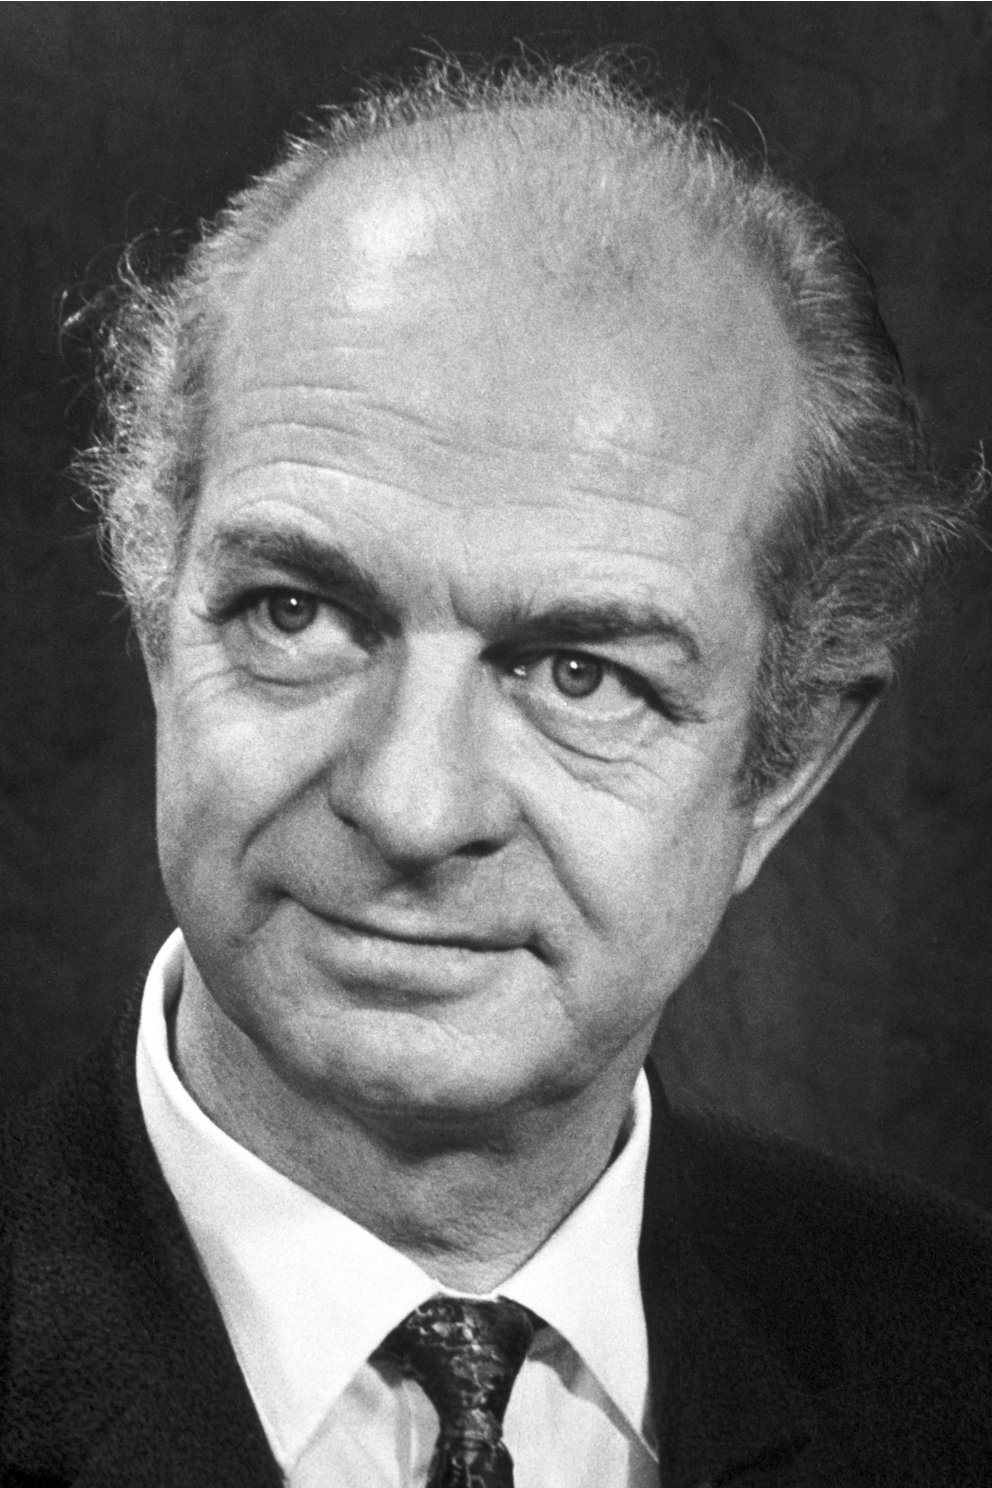
\includegraphics[width=0.26\linewidth]{images/book3/pauling.jpg}

{\small लाइनस पॉलिंग (1901--1994), जिन्होंने \omterm{def:b1:proteins:peptide}{पेप्टाइड बंध} की समतलता और
\omterm{def:b1:water-small-molecules:water}{हाइड्रोजन बंधों} की ज्यामिति से 1951 में $\alpha$ कुंडली तथा
$\beta$ पट्ट निकाल लिए, इससे पहले कि इनमें से कोई किसी \omterm{def:b1:proteins:peptide}{प्रोटीन} में देखा
गया हो। छायाचित्र: नोबेल फ़ाउंडेशन, 1962, सार्वजनिक अधिकार-मुक्त।}
\end{omfigure}

\begin{example}[संख्याओं में कुंडली और पट्ट]\label{ex:b1:proteins:numbers}
झिल्ली पार करती किसी $\alpha$ कुंडली को \qty{3}{nm} का जलविरागी
अंतर्भाग पार करना पड़ता है: $3/0.15 = 20$ अवशेष, और सचमुच
\cref{ch:b1:membranes-transport} के अंतःझिल्ली खंड लगभग बीस जलविरागी
अवशेषों की लड़ियाँ हैं। उतनी ही लंबाई की कोई $\beta$ लड़ी
\qty{7}{nm} तक फैलती है: रेशम का फ़ाइब्रोइन ग्लाइसीन और ऐलानीन के चिने
हुए प्रतिसमांतर पट्ट है, और रेशम का धागा उतने ही भार के इस्पात से अधिक
मज़बूत है, क्योंकि सहसंयोजी रीढ़ें तंतु की दिशा में ही लेटी हैं।
\end{example}

\section{तृतीयक और चतुष्क संरचना}

\begin{definition}[तृतीयक और चतुष्क संरचना]\label{def:b1:proteins:tertiary}
\emph{तृतीयक संरचना}\index{तृतीयक संरचना} किसी एक \omterm{def:b1:proteins:peptide}{बहुपेप्टाइड} की पूरी
त्रिविम सजावट है: उसकी कुंडलियाँ, पट्ट और फंदे आपस में जमे हुए, और
प्रायः कई ऐसे संहत \emph{प्रांतों} में जो स्वतंत्र रूप से मुड़ते हैं।
उसे असहसंयोजी बल थामते हैं --- \emph{\omterm{prop:b1:water-small-molecules:properties}{जलविरागी प्रभाव}}, जो अध्रुवीय
\omterm{def:b1:proteins:aminoacid}{पार्श्व शृंखलाओं} को जल से दूर किसी अंतर्भाग में गाड़ देता है, \omterm{def:b1:water-small-molecules:water}{हाइड्रोजन
बंध}, आवेशित \omterm{def:b1:proteins:aminoacid}{पार्श्व शृंखलाओं} के बीच लवण-सेतु, और \omterm{def:b1:water-small-molecules:bonds}{वान डर वाल्स} जमाव ---
और कभी-कभी \emph{डाइसल्फ़ाइड सेतु}\index{डाइसल्फ़ाइड सेतु}, यानी दो
सिस्टीनों के बीच सहसंयोजी S--S बंध, उन \omterm{def:b1:proteins:peptide}{प्रोटीनों} में जो ऑक्सीकारक बाहर की
ओर स्रावित होते हैं। \emph{चतुष्क संरचना}\index{चतुष्क संरचना} कई
बहुपेप्टाइडों (उपइकाइयों) का एक ही \omterm{def:b1:proteins:peptide}{प्रोटीन} में जुड़ना है:
हीमोग्लोबिन दो $\alpha$ और दो $\beta$ शृंखलाएँ हैं। \emph{गोलिकाकार}
\omterm{def:b1:proteins:peptide}{प्रोटीन} संहत और जल-घुलनशील होते हैं (एंजाइम, वाहक);
\emph{तंतुमय} \omterm{def:b1:proteins:peptide}{प्रोटीन} फैले हुए और अघुलनशील (\omterm{def:b1:body-plans-tissues:connective}{कोलैजन} की तिहरी
कुंडली, केराटिन तथा मायोसिन की कुंडलित कुंडलियाँ, रेशम)।
\end{definition}

\begin{omfigure}
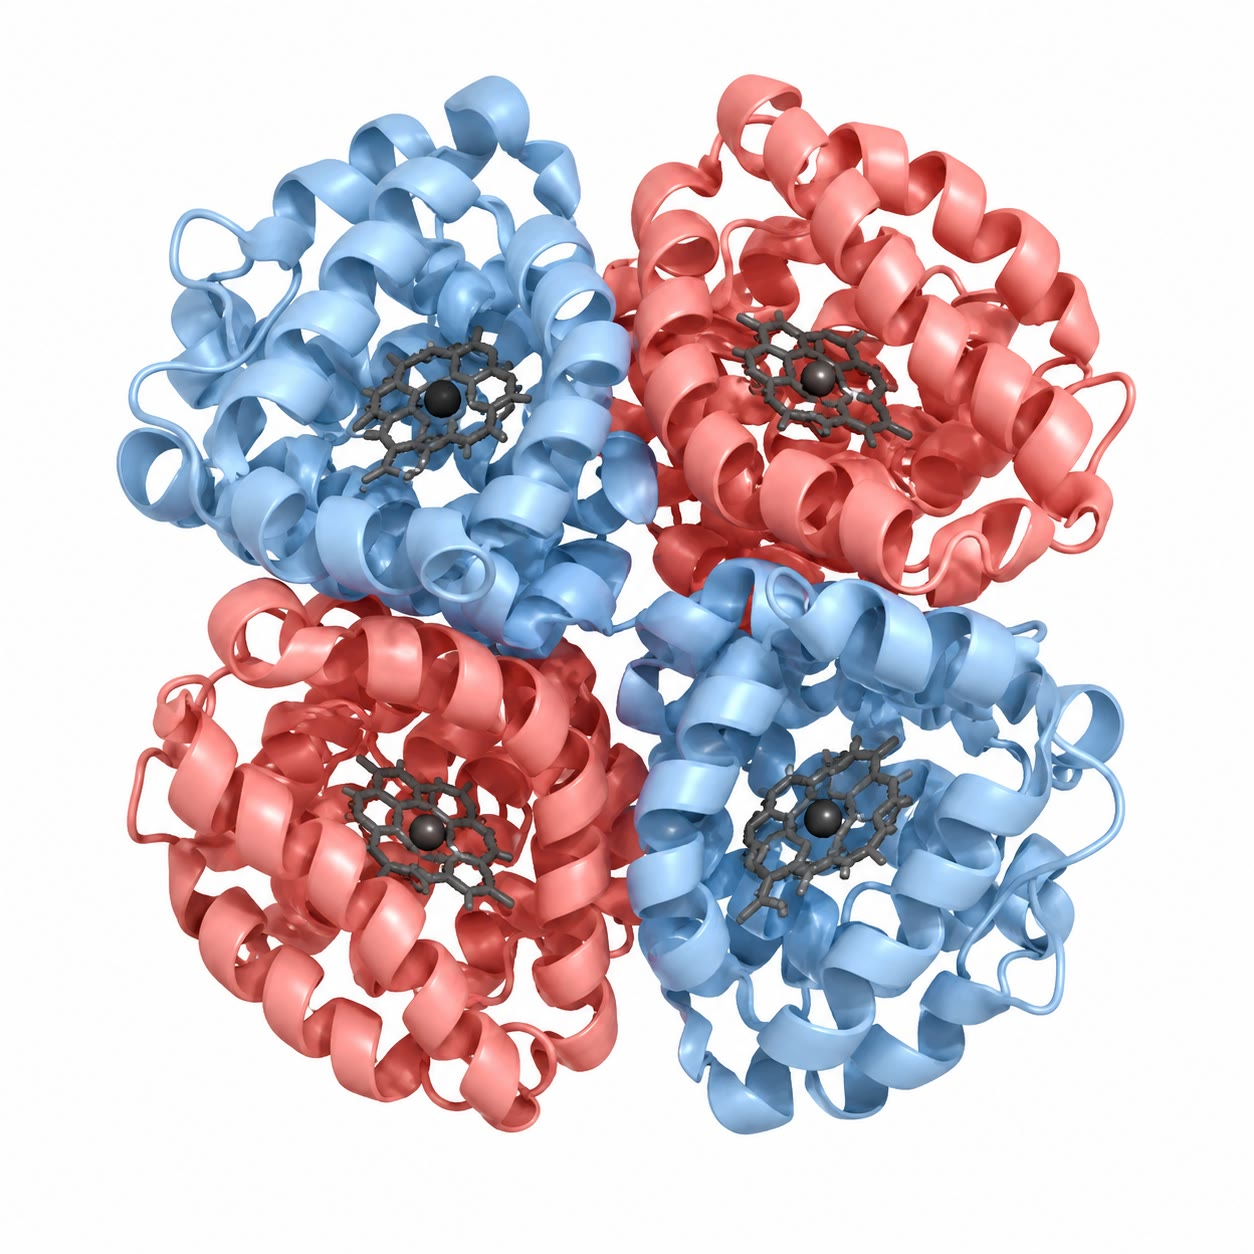
\includegraphics[width=0.42\linewidth]{images/book3/ai/fig-hemoglobin-ribbon.jpg}

{\small हीमोग्लोबिन: चार उपइकाइयाँ, दो $\alpha$ (नीली) और दो $\beta$
(लाल), और हर एक किसी हीम समूह (गहरा) के चारों ओर $\alpha$ कुंडलियों का
गुच्छा, जिसका लोहा एक $\mathrm{O_2}$ बाँधता है। चारों स्थल स्वतंत्र रूप
से काम नहीं करते।}
\end{omfigure}

\begin{theorem}[अनुक्रम ही वलन तय करता है]\label{thm:b1:proteins:anfinsen}
\index{प्रोटीन वलन}
किसी \omterm{def:b1:proteins:peptide}{प्रोटीन} की त्रिविम संरचना उसके ऐमीनो-अम्ल अनुक्रम से तय होती है:
मूल वलन वह संरूपण है जिसकी \omterm{prop:b1:water-small-molecules:gibbs}{मुक्त ऊर्जा} उन सब संरूपणों में सबसे कम है
जिन तक शृंखला अपने कोशिकीय परिवेश में पहुँच सकती है, और उस तक पहुँचने के
लिए चाहिए जानकारी स्वयं शृंखला में है।
\end{theorem}
\begin{proof}[साक्ष्य]
ऐन्फ़िन्सन (1961) ने राइबोन्यूक्लिएज़ A को, जो चार \omterm{def:b1:proteins:tertiary}{डाइसल्फ़ाइड सेतुओं}
वाला \qty{124}{}-अवशेषी एंजाइम है, गाढ़े यूरिया में ऐसे अपचायक के साथ
खोला जिसने वे सेतु तोड़ दिए: शृंखला की सारी क्रियाशीलता चली गई। यूरिया
हटाकर और सिस्टीनों को हवा में धीरे-धीरे फिर ऑक्सीकृत होने देकर उन्होंने
एंजाइम पूरी क्रियाशीलता के साथ वापस पाया, जिसके चारों सेतु उन्हीं आठ
सिस्टीनों के बीच \qty{105}{} संभव युग्मनों में से फिर बन चुके थे ---
शृंखला ने अपना वलन स्वयं ढूँढ़ लिया था। यूरिया में रहते हुए ही फिर
ऑक्सीकृत करने पर उसने यादृच्छिक सेतु बनाए और निष्क्रिय रही; फिर अपचायक की
एक बूँद ने उसे तब तक उन्हें फेंटने दिया जब तक मूल समुच्चय, जो सबसे
स्थायी है, न मिल गया। तब से हज़ारों अनुक्रम परखनली में शून्य से मोड़े जा
चुके हैं, और किसी नए अनुक्रम का वलन अब उसी से गणना किया जा सकता है।
\end{proof}

\begin{proposition}[विकृतीकरण]\label{prop:b1:proteins:denaturation}
\index{विकृतीकरण (प्रोटीन)}
ऊष्मा, चरम pH, यूरिया, अपमार्जक या कार्बनिक विलायक उन दुर्बल बंधों पर
भारी पड़कर \omterm{def:b1:proteins:peptide}{प्रोटीन} खोल देते हैं जो वलन थामे रहते हैं: शृंखला अपनी आकृति
और अपना कार्य खो देती है, अपना जलविरागी अंतर्भाग उघाड़ देती है, और अपने
पड़ोसियों से गुत्थम-गुत्था हो जाती है। छोटे \omterm{def:b1:proteins:peptide}{प्रोटीन} विकृतकारी हटते ही फिर
मुड़ जाते हैं; बड़े \omterm{def:b1:proteins:peptide}{प्रोटीन}, और किसी भीड़-भरी \omterm{def:b1:cell-unit-of-life:cell}{कोशिका} के \omterm{def:b1:proteins:peptide}{प्रोटीन}, प्रायः
नहीं मुड़ पाते, और \omterm{def:b1:cell-unit-of-life:cell}{कोशिका} \emph{परिचारक}\index{परिचारक} रखती है ---
यानी वे \omterm{def:b1:proteins:peptide}{प्रोटीन} जो खुली शृंखलाओं से बँधते हैं, उनकी जलविरागी सतहें ढाँप
लेते हैं, और उन्हें ठीक मुड़ने के बार-बार अवसर देते हैं --- और जो ग़लत
मुड़ा रह जाए उसे नष्ट कर देती है। कुछ डिग्री का ज्वर, और वह
\qty{42}{\celsius} जिस पर मस्तिष्क के \omterm{def:b1:proteins:peptide}{प्रोटीन} खुलने लगते हैं, स्थायित्व
की सँकरी सीमा दिखाते हैं: कोई प्रारूपिक वलन खुली शृंखला से केवल
\qtyrange{20}{60}{kJ/mol} अधिक स्थायी होता है, यानी कुछ ही \omterm{def:b1:water-small-molecules:water}{हाइड्रोजन
बंधों} जितना।
\end{proposition}

\begin{omfigure}
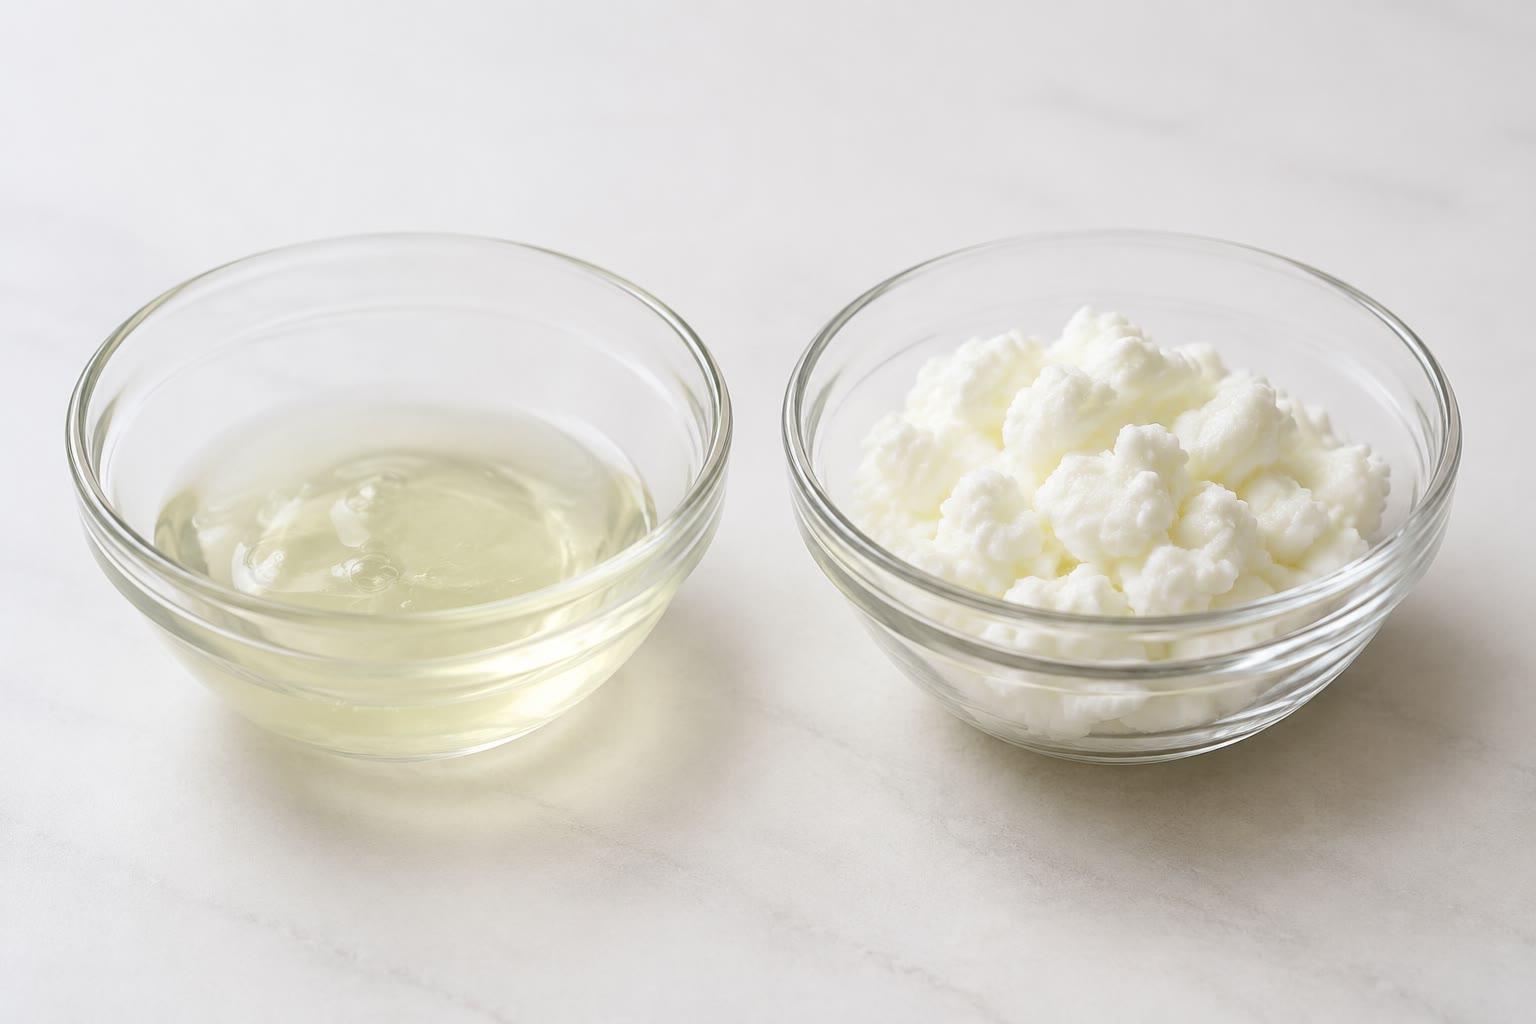
\includegraphics[width=0.5\linewidth]{images/book3/ai/b3-12-egg-white-cooked.jpg}

{\small कच्चा और पका अंडे का सफ़ेद भाग: वही \omterm{def:b1:proteins:peptide}{प्रोटीन}, बाएँ मुड़े हुए और
घुलनशील, दाएँ खुले हुए और किसी अपारदर्शी ठोस में गुत्थे हुए। ऊष्मा के
सिवा कुछ नहीं जोड़ा गया।}
\end{omfigure}

\begin{example}[कोलैजन]\label{ex:b1:proteins:collagen}
किसी स्तनधारी के \omterm{def:b1:proteins:peptide}{प्रोटीन} का एक-चौथाई \omterm{def:b1:body-plans-tissues:connective}{कोलैजन} है: तीन शृंखलाएँ, जिनमें से
हर एक एक हज़ार अवशेषों की वामावर्त कुंडली है जिसमें हर तीसरे स्थान पर
ग्लाइसीन है (ग्लाइ--X--Y, जिसमें Y प्रायः हाइड्रॉक्सीप्रोलीन है), और जो
आपस में लिपटकर \qty{300}{nm} लंबी एक दक्षिणावर्त तिहरी कुंडली बनाती हैं,
और फिर अगल-बगल जमकर ऐसे तंतुक बनाती हैं जिन्हें \omterm{def:b1:water-small-molecules:bonds}{सहसंयोजी बंध} आपस में
बाँधते हैं। ग्लाइसीन में \omterm{def:b1:proteins:aminoacid}{पार्श्व शृंखला} का न होना ही तीनों शृंखलाओं को
अक्ष पर जमने देता है; और ग्लाइसीन की जगह किसी और अवशेष का एक ही
प्रतिस्थापन कुंडली में मोड़ डाल देता है और हड्डियाँ भुरभुरी कर देता है।
प्रोलीनों के हाइड्रॉक्सिलीकरण के लिए विटामिन C चाहिए; उसके बिना कुंडली
अस्थिर रहती है और तंतुक चूक जाते हैं: स्कर्वी।
\end{example}

\section{अन्यस्थानिकता: हीमोग्लोबिन}

\begin{definition}[अन्यस्थानिकता, सहकारिता]\label{def:b1:proteins:allostery}
कोई \omterm{def:b1:proteins:peptide}{प्रोटीन} \emph{अन्यस्थानिक}\index{अन्यस्थानिकता} तब है जब किसी एक
स्थल पर किसी बंधक का बँधना \omterm{def:b1:proteins:peptide}{प्रोटीन} का संरूपण बदल दे और उससे किसी दूसरे
स्थल पर उसकी बंधुता भी। जब स्थल एक जैसे हों और वह परिवर्तन बाक़ी की
बंधुता बढ़ाता हो, तब बंधन \emph{सहकारी}\index{सहकारिता} है:
संतृप्ति वक्र अतिपरवलय के बजाय अंग्रेज़ी S जैसा हो जाता है, और \omterm{def:b1:proteins:peptide}{प्रोटीन}
बंधक की सांद्रता के किसी सँकरे परास में लगभग ख़ाली से लगभग भरा हो जाता
है। \emph{हिल समीकरण}\index{हिल समीकरण} इसका वर्णन करता है:
\[
Y = \frac{P^n}{P_{50}^n + P^n},
\]
जिसमें $Y$ घिरे हुए स्थलों का भिन्न है, $P$ बंधक की सांद्रता
(या आंशिक दाब), $P_{50}$ आधी संतृप्ति पर उसका मान, और $n$ हिल गुणांक ---
स्वतंत्र स्थलों के लिए 1, और पूर्ण सहकारिता के लिए स्थलों की संख्या तक।
\end{definition}

\begin{proposition}[हीमोग्लोबिन और मायोग्लोबिन]\label{prop:b1:proteins:hemoglobin}
मायोग्लोबिन, जो एक हीम वाली एक ही शृंखला है, $\mathrm{O_2}$ को किसी
अतिपरवलय के साथ बाँधता है ($n = 1$, $P_{50} = \qty{0.37}{kPa}$): \omterm{def:b1:body-plans-tissues:tissue}{ऊतक} जो
भी दाब दें उस पर वह संतृप्त रहता है और पेशी में भंडार का काम करता है।
हीमोग्लोबिन, जो चार उपइकाइयाँ हैं, \omterm{def:b1:proteins:allostery}{सहकारी} रूप से बाँधता है ($n \approx 2.8$,
$P_{50} = \qty{3.5}{kPa}$): पहला बँधा $\mathrm{O_2}$ उस
चतुष्क को कम-बंधुता वाली \emph{T अवस्था} से अधिक-बंधुता वाली
\emph{R अवस्था} की ओर खिसका देता है, इसलिए वह फेफड़े के
\qty{13}{kPa} पर लगभग पूरा भर जाता है और \omterm{def:b1:body-plans-tissues:tissue}{ऊतकों} के
\qty{5}{kPa} पर एक बड़ा भिन्न उतार देता है। उसकी बंधुता अम्ल और
$\mathrm{CO_2}$ से (\emph{बोर प्रभाव}) तथा
2,3-बिसफ़ॉस्फ़ोग्लिसरेट (BPG) से और घट जाती है, जो T अवस्था से बँधता है,
और इससे उतारना आसान हो जाता है: काम करती किसी पेशी में, या ऊँचाई पर, उसी
दाब पर अधिक ऑक्सीजन छूटती है। भ्रूण ऐसा हीमोग्लोबिन बनाता है जो BPG को
कमज़ोर बाँधता है, इसलिए उसका रक्त अपरा के आरपार माता के रक्त से ऑक्सीजन
खींच लेता है।
\end{proposition}

\begin{omfigure}
\begin{tikzpicture}
\begin{axis}[
  width=0.9\linewidth, height=6.4cm,
  axis x line=bottom, axis y line=left,
  xmin=0, xmax=14, ymin=0, ymax=1.08,
  xlabel={$\mathrm{O_2}$ का आंशिक दाब (\unit{kPa})}, ylabel={घिरे हुए स्थलों का भिन्न $Y$},
  xlabel style={font=\small, at={(axis description cs:0.5,-0.12)}, anchor=north},
  ylabel style={font=\small},
  tick label style={font=\small}, xtick={0,2,4,6,8,10,12,14}, ytick={0,0.25,0.5,0.75,1},
  legend style={font=\small, at={(0.97,0.35)}, anchor=north east, draw=none},
  clip=false,
]
\addplot[very thick, omDef, domain=0.01:14, samples=120] {x/(0.37+x)};
\addlegendentry{मायोग्लोबिन, $n=1$, $P_{50} = \qty{0.37}{kPa}$}
\addplot[very thick, omThm, domain=0.01:14, samples=120] {x^2.8/(3.5^2.8+x^2.8)};
\addlegendentry{हीमोग्लोबिन, $n=2.8$, $P_{50} = \qty{3.5}{kPa}$}
\addplot[very thick, omProp, dashed, domain=0.01:14, samples=120] {x^2.8/(4.5^2.8+x^2.8)};
\addlegendentry{अम्ल में हीमोग्लोबिन, $P_{50} = \qty{4.5}{kPa}$ (बोर)}
\draw[dashed, gray] (axis cs:13.3,0) -- (axis cs:13.3,1.0); \node[font=\scriptsize, anchor=south] at (axis cs:13.3,1.01) {फेफड़े};
\draw[dashed, gray] (axis cs:5.3,0) -- (axis cs:5.3,0.76); \node[font=\scriptsize, anchor=west] at (axis cs:5.45,0.07) {ऊतक};
\end{axis}
\end{tikzpicture}

{\small मायोग्लोबिन (अतिपरवलयी) और हीमोग्लोबिन (S जैसा) द्वारा ऑक्सीजन का
बंधन। फेफड़ों और \omterm{def:b1:body-plans-tissues:tissue}{ऊतकों} के बीच मायोग्लोबिन लगभग कुछ नहीं छोड़ता;
हीमोग्लोबिन अपने भार का पाँचवाँ भाग छोड़ता है, और \omterm{def:b1:body-plans-tissues:tissue}{ऊतक} के अम्लीय होने पर
उससे भी अधिक।}
\end{omfigure}

\begin{method}[हिल समीकरण का उपयोग]\label{met:b1:proteins:hill}
\begin{enumerate}
  \item $P_{50}$ को वक्र से $Y = 0.5$ पर पढ़िए; और $n$ को
        $\log[Y/(1-Y)]$ की उस प्रवणता से आँकिए जो $\log P$ के सापेक्ष
        है (हिल आलेख), और जो $n$ प्रवणता की एक सरल रेखा है, $P_{50}$
        के पास।
  \item भरने के दाब (फेफड़े) पर और उतारने के दाब (\omterm{def:b1:body-plans-tissues:tissue}{ऊतक}) पर $Y$
        निकालिए; उनका अंतर ही वहन-क्षमता का वह भिन्न है जो पहुँचाया
        जाता है।
  \item उसे क्षमता से गुणा कीजिए: रक्त में \qty{150}{g/L}
        हीमोग्लोबिन है, और हर ग्राम \qty{1.34}{mL} $\mathrm{O_2}$
        बाँधता है, यानी संतृप्त होने पर प्रति लीटर \qty{200}{mL} $\mathrm{O_2}$।
  \item बोर प्रभाव या BPG को गिनने के लिए खिसका हुआ $P_{50}$ केवल
        \omterm{def:b1:body-plans-tissues:tissue}{ऊतकों} पर लगाइए, जहाँ अम्ल है।
\end{enumerate}
\end{method}

\section{प्रोटीन देखना और अलग करना}

\begin{method}[प्रोटीन अलग करना]\label{met:b1:proteins:methods}
\begin{enumerate}
  \item \emph{SDS में वैद्युतकणसंचलन}: यह अपमार्जक हर शृंखला को उसकी
        लंबाई के समानुपात में ऋण आवेश से लेप देता है, इसलिए शृंखलाएँ
        किसी पॉलिऐक्रिलामाइड जेल में केवल आकार से चलती हैं; ज्ञात
        द्रव्यमानों की एक सीढ़ी जेल को अंशांकित करती है, और किसी रंगी
        पट्टी की स्थिति द्रव्यमान कुछ प्रतिशत तक दे देती है।
  \item \emph{वर्णलेखन}: मनकों के किसी स्तंभ से होकर, जो \omterm{def:b1:proteins:peptide}{प्रोटीनों} को
        आकार से रोकते हैं (जेल निस्यंदन: बड़े पहले निकलते हैं), आवेश से
        (आयन विनिमय), या विशिष्ट बंधन से (बंधुता: कोई जड़ा हुआ बंधक एक
        \omterm{def:b1:proteins:peptide}{प्रोटीन} थाम लेता है और बाक़ी को निकल जाने देता है)।
        किसी शुद्धीकरण का पीछा विशिष्ट क्रिया के बढ़ने से किया जाता है
        (\cref{ch:b1:cell-unit-of-life})।
  \item \emph{अनुक्रमण}: जीन का अनुक्रम, अनूदित करके; या स्वयं \omterm{def:b1:proteins:peptide}{प्रोटीन},
        पेप्टाइडों में काटकर और द्रव्यमान स्पेक्ट्रमिकी से पढ़कर।
  \item \emph{संरचना}: किसी क्रिस्टल का X-किरण विवर्तन, या जमे हुए एकल
        कणों की इलेक्ट्रॉन सूक्ष्मदर्शिकी, हर परमाणु की स्थिति दे देती
        है; और इस अध्याय के फ़ीता-चित्र उन्हीं के सार हैं।
\end{enumerate}
\end{method}

\begin{omfigure}
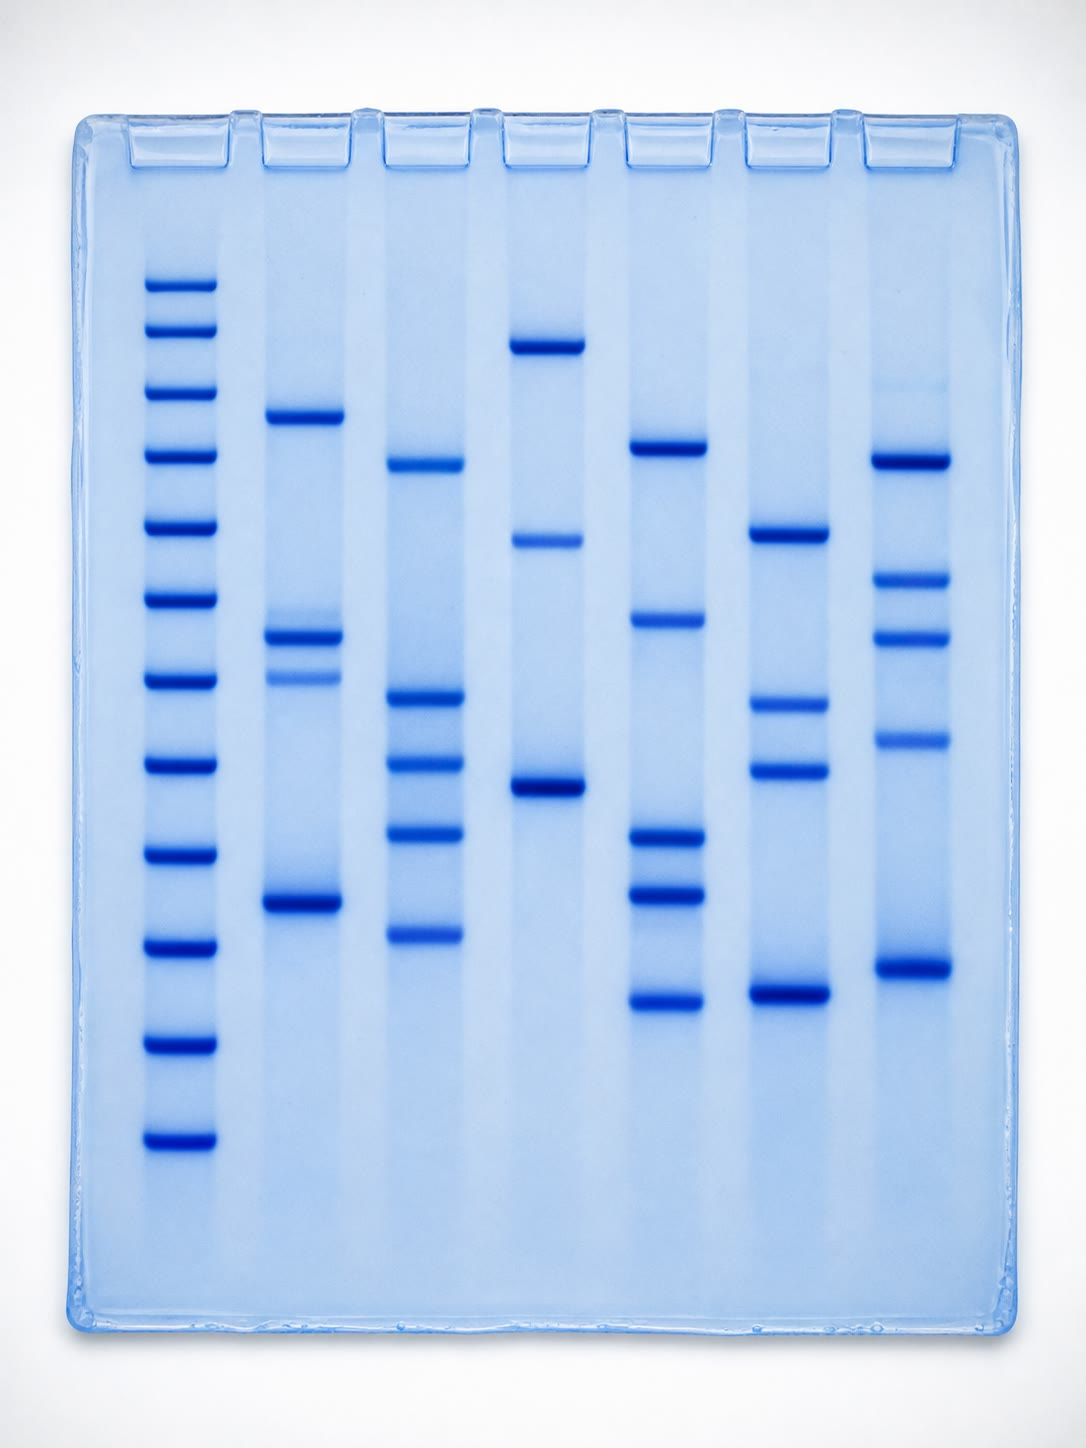
\includegraphics[width=0.36\linewidth]{images/book3/ai/b3-12-protein-gel.jpg}

{\small एक रंगा हुआ SDS--पॉलिऐक्रिलामाइड जेल। हर लेन एक नमूना है; हर
पट्टी एक ही आकार का \omterm{def:b1:proteins:peptide}{प्रोटीन}; और बाईं लेन ज्ञात द्रव्यमान के सूचकों की
सीढ़ी। छोटे \omterm{def:b1:proteins:peptide}{प्रोटीन} दूर तक दौड़ते हैं।}
\end{omfigure}

\begin{example}[कोई जेल पढ़ना]\label{ex:b1:proteins:gel}
किसी कच्चे निष्कर्ष में दर्जनों पट्टियाँ दिखती हैं; बंधुता वर्णलेखन के
बाद \qty{33}{kDa} सूचक की स्थिति पर एक ही पट्टी बचती है। SDS के बिना और
अपचायक के बिना चलाने पर वही \omterm{def:b1:proteins:peptide}{प्रोटीन} \qty{66}{kDa} की स्पीशीज़ के रूप में
चलता है: वह दो एक जैसी शृंखलाओं का द्विलक है जिन्हें कोई \omterm{def:b1:proteins:tertiary}{डाइसल्फ़ाइड
सेतु} थामे है, और जिसे अपचायक तोड़ देता है तथा अपमार्जक अलग कर देता है।
दो जेल, तर्क की एक ही लड़ी, और \omterm{def:b1:proteins:tertiary}{चतुष्क संरचना} पता चल जाती है।
\end{example}

\section{अभ्यास}

\begin{exercise}[$\star$]\label{exo:b1:proteins:1}
pH 7 पर किसी \omterm{def:b1:proteins:aminoacid}{ऐमीनो अम्ल} की सामान्य संरचना बनाइए या उसका वर्णन कीजिए, और
Leu, Ser, Lys, Glu तथा Phe को \omterm{def:b1:proteins:aminoacid}{पार्श्व शृंखला} से वर्गीकृत कीजिए।
\end{exercise}

\begin{exercise}[$\star$]\label{exo:b1:proteins:2}
\omterm{def:b1:proteins:peptide}{प्रोटीन} संरचना के चारों स्तर और हर एक को थामने वाले बंध बताइए।
\end{exercise}

\begin{exercise}[$\star$]\label{exo:b1:proteins:3}
किसी \omterm{def:b1:proteins:peptide}{प्रोटीन} में \qty{450}{} अवशेष हैं। उसका द्रव्यमान आँकिए। यदि वह एक
ही $\alpha$ कुंडली होता तो कितना लंबा होता? और एक ही $\beta$ लड़ी होता तो?
\end{exercise}

\begin{exercise}[$\star$]\label{exo:b1:proteins:4}
ऑक्सीजन-बंधन वाले आलेख से \qty{13.3}{kPa} पर और \qty{5.3}{kPa} पर
हीमोग्लोबिन की संतृप्ति, और पहुँचाया गया भिन्न पढ़िए।
\end{exercise}

\begin{exercise}[$\star\star$]\label{exo:b1:proteins:5}
अध्याय के p$K_a$ मानों से पेप्टाइड Lys--Gly--Asp--Ala का शुद्ध आवेश pH 7
पर, pH 2 पर और pH 12 पर निकालिए, और उसका \omterm{prop:b1:proteins:ionisation}{सम-विद्युत बिंदु} आँकिए।
\end{exercise}

\begin{exercise}[$\star\star$]\label{exo:b1:proteins:6}
रीढ़ की ज्यामिति से समझाइए कि प्रोलीन $\alpha$ कुंडलियों के भीतर कम
क्यों मिलता है और ग्लाइसीन तंग मोड़ों पर क्यों।
\end{exercise}

\begin{exercise}[$\star\star$]\label{exo:b1:proteins:7}
ऐन्फ़िन्सन के प्रयोग में यादृच्छिक पुनःऑक्सीकरणों का कितना भिन्न
डाइसल्फ़ाइडों का मूल समुच्चय देता? (आठ सिस्टीनों के युग्मन के ढंग
गिनिए।) पूरी क्रियाशीलता की वास्तविक वापसी ने क्या सिद्ध किया?
\end{exercise}

\begin{exercise}[$\star\star$]\label{exo:b1:proteins:8}
$n = 2.8$ और $P_{50} = \qty{3.5}{kPa}$ के साथ \omterm{def:b1:proteins:allostery}{हिल समीकरण} से
\qty{2}{kPa}, \qty{3.5}{kPa} और \qty{8}{kPa} पर $Y$ निकालिए। फिर
$n = 1$ के साथ वही दोहराइए। \qty{8}{} और \qty{2}{kPa} के बीच कौन-सा
\omterm{def:b1:proteins:peptide}{प्रोटीन} अधिक पहुँचाता है?
\end{exercise}

\begin{exercise}[$\star\star$]\label{exo:b1:proteins:9}
कोई \omterm{def:b1:proteins:peptide}{प्रोटीन} किसी SDS जेल पर \qty{50}{kDa} की एक ही पट्टी के रूप में
चलता है और किसी जेल-निस्यंदन स्तंभ से \qty{200}{kDa} पर निकलता है। उसकी
\omterm{def:b1:proteins:tertiary}{चतुष्क संरचना} बताइए और यह भी कि उपइकाइयों के बीच \omterm{def:b1:proteins:tertiary}{डाइसल्फ़ाइड सेतुओं} की
जाँच आप कैसे करेंगे।
\end{exercise}

\begin{exercise}[$\star\star\star$]\label{exo:b1:proteins:10}
हँसियाकार-कोशिका हीमोग्लोबिन में $\beta$ शृंखला की सतह पर स्थिति 6 पर
ग्लूटामेट की जगह वैलीन है। दोनों \omterm{def:b1:proteins:aminoacid}{पार्श्व शृंखलाओं} के रसायन से समझाइए कि
ऑक्सीजन उतरने पर उत्परिवर्ती \omterm{def:b1:proteins:peptide}{प्रोटीन} बहुलकित क्यों हो जाता है, और यह रोग
फेफड़ों के बजाय \omterm{def:b1:body-plans-tissues:tissue}{ऊतकों} में क्यों दिखता है।
\end{exercise}

\begin{exercise}[$\star\star\star$]\label{exo:b1:proteins:11}
कोई वलन केवल \qty{40}{kJ/mol} से स्थायी है। \qty{37}{\celsius} पर साम्य
में खुले अणुओं का भिन्न निकालिए ($K = e^{-\Delta G/RT}$),
और \qty{45}{\celsius} पर भी यदि $\Delta G$ गिरकर
\qty{10}{kJ/mol} हो जाए। इतना सीमांत स्थायित्व किसी \omterm{def:b1:cell-unit-of-life:cell}{कोशिका} के काम का
क्यों है?
\end{exercise}

\begin{exercise}[$\star\star\star$]\label{exo:b1:proteins:12}
``\omterm{def:b1:proteins:peptide}{प्रोटीन} वह अनुक्रम है जो किसी आकृति में मुड़ जाता है, और आकृति ही
कार्य है।'' ऐन्फ़िन्सन, परिचारकों, हँसियाकार \omterm{def:b1:cell-unit-of-life:cell}{कोशिका} और \omterm{def:b1:proteins:allostery}{अन्यस्थानिकता} के
साथ एक अनुच्छेद में चर्चा कीजिए: यह वाक्य कहाँ टिकता है और कहाँ \omterm{def:b1:cell-unit-of-life:cell}{कोशिका} को
हस्तक्षेप करना पड़ता है।
\end{exercise}

\section{समस्या: काम पर हीमोग्लोबिन}

\begin{problem}[{सप्ताहांत समस्या --- फेफड़े से पेशी तक ढोई गई
ऑक्सीजन, विश्राम में, किसी दौड़ में, किसी पहाड़ पर और जन्म से पहले, और
अंत में प्रति लीटर रक्त पहुँचाई गई ऑक्सीजन}]
\label{pb:b1:proteins:1}
रक्त में \qty{150}{g/L} हीमोग्लोबिन है; \qty{1}{g}
\qty{1.34}{mL} $\mathrm{O_2}$ बाँधता है। हीमोग्लोबिन pH 7.4 पर
$n = 2.8$ और $P_{50} = \qty{3.5}{kPa}$ के साथ \omterm{def:b1:proteins:allostery}{हिल समीकरण} मानता है;
मायोग्लोबिन का $n = 1$ और $P_{50} = \qty{0.37}{kPa}$ है।
$\mathrm{O_2}$ के आंशिक दाब: समुद्र-तल पर फेफड़ों में \qty{13.3}{kPa},
विश्राम कर रहे \omterm{def:b1:body-plans-tissues:tissue}{ऊतकों} में \qty{5.3}{kPa}। $2.8\ln 3.5 = 3.51$,
$2.8\ln 5.3 = 4.67$, $2.8\ln 13.3 = 7.25$, $2.8\ln 2.7 = 2.78$,
$2.8\ln 4.5 = 4.21$, $2.8\ln 7 = 5.45$, $2.8\ln 4 = 3.88$,
$2.8\ln 2.6 = 2.68$ लीजिए।

\medskip
\noindent\textbf{भाग I --- विश्राम में।}
\begin{enumerate}
  \item एक लीटर रक्त की ऑक्सीजन-क्षमता निकालिए।
  \item $P^{2.8}$ निकालिए, $P = 3.5$, $5.3$ और $13.3$ kPa के लिए
        ($e^{2.8\ln P}$ के रूप में)।
  \item फेफड़ों में और \omterm{def:b1:body-plans-tissues:tissue}{ऊतकों} में हीमोग्लोबिन की संतृप्ति $Y$ निकालिए।
  \item भार का पहुँचाया गया भिन्न और प्रति लीटर रक्त पहुँचाई गई ऑक्सीजन
        मिलीलीटर में निकालिए।
  \item विश्राम कर रहा कोई मनुष्य प्रति मिनट \qty{250}{mL}
        $\mathrm{O_2}$ खपाता है। इस आपूर्ति के लिए कितना हृदय-निर्गम
        चाहिए?
  \item उन्हीं दोनों दाबों पर मायोग्लोबिन की संतृप्ति और, यदि वह
        हीमोग्लोबिन की जगह होता तो, प्रति लीटर पहुँचाई गई ऑक्सीजन
        निकालिए। निष्कर्ष निकालिए।
  \item एक वाक्य में समझाइए कि \omterm{def:b1:proteins:allostery}{सहकारिता} क्या कमा देती है।
\end{enumerate}

\medskip
\noindent\textbf{भाग II --- एक दौड़।}
दौड़ती किसी पेशी में pH गिरकर 7.2 हो जाता है और $\mathrm{O_2}$ का
स्थानीय दाब \qty{2.7}{kPa}; और बोर प्रभाव वहाँ $P_{50}$ बढ़ाकर
\qty{4.5}{kPa} कर देता है।
\begin{enumerate}[resume]
  \item $Y$ निकालिए \qty{2.7}{kPa} पर, $P_{50} = \qty{3.5}{kPa}$
        के साथ (बिना बोर प्रभाव के)।
  \item $Y$ निकालिए \qty{2.7}{kPa} पर, $P_{50} = \qty{4.5}{kPa}$
        के साथ।
  \item दोनों स्थितियों में प्रति लीटर पहुँचाई गई ऑक्सीजन निकालिए
        (फेफड़ों में भरना अपरिवर्तित) और बोर प्रभाव से हुई कमाई भी।
  \item पेशी का मायोग्लोबिन $P = \qty{2.7}{kPa}$ पर है। उसकी संतृप्ति
        क्या है, और किसी संकुचन के दौरान दाब गिरकर
        \qty{0.5}{kPa} हो जाए तो उसका क्या होता है?
  \item समझाइए कि बोर प्रभाव \omterm{def:b1:proteins:allostery}{अन्यस्थानिकता} का ही एक रूप क्यों है और
        प्रोटॉन कहाँ क्रिया करते हैं।
\end{enumerate}

\medskip
\noindent\textbf{भाग III --- एक पहाड़।}
\qty{4000}{m} पर फेफड़ों का $\mathrm{O_2}$ दाब \qty{7}{kPa} है।
दिनों के भीतर लाल \omterm{def:b1:cell-unit-of-life:cell}{कोशिकाएँ} अपना BPG बढ़ा लेती हैं और $P_{50}$
\qty{4.0}{kPa} पर खिसका देती हैं; और हफ़्तों के भीतर मज्जा हीमोग्लोबिन
\qty{180}{g/L} तक बढ़ा देती है।
\begin{enumerate}[resume]
  \item $P_{50} = \qty{3.5}{kPa}$ के साथ \qty{7}{kPa} पर फेफड़ों की
        संतृप्ति और प्रति लीटर आपूर्ति निकालिए (\omterm{def:b1:body-plans-tissues:tissue}{ऊतक}
        \qty{5.3}{kPa} पर)। समुद्र-तल से तुलना कीजिए।
  \item $P_{50} = \qty{4.0}{kPa}$ के साथ फेफड़े और \omterm{def:b1:body-plans-tissues:tissue}{ऊतक} की संतृप्तियाँ,
        तथा आपूर्ति निकालिए।
  \item समझाइए कि बंधुता घटाने से मदद क्यों मिलती है, जबकि उससे
        फेफड़ों में भरना घट जाता है।
  \item $P_{50} = \qty{4.0}{kPa}$ और \qty{180}{g/L} हीमोग्लोबिन के साथ
        प्रति लीटर आपूर्ति निकालिए।
  \item क्या इससे भी कम बंधुता ($P_{50} = \qty{6}{kPa}$) \qty{7}{kPa}
        पर मदद करती? दोनों संतृप्तियाँ निकालिए और निर्णय कीजिए।
\end{enumerate}

\medskip
\noindent\textbf{भाग IV --- जन्म से पहले।}
भ्रूणीय हीमोग्लोबिन का $P_{50} = \qty{2.6}{kPa}$ है; और अपरा में
$\mathrm{O_2}$ का दाब दोनों ओर \qty{4}{kPa} है।
\begin{enumerate}[resume]
  \item \qty{4}{kPa} पर माता के हीमोग्लोबिन की संतृप्ति निकालिए।
  \item \qty{4}{kPa} पर भ्रूणीय हीमोग्लोबिन की संतृप्ति निकालिए।
  \item समझाइए कि दोनों ओर दाब एक ही होते हुए भी ऑक्सीजन माता से भ्रूण
        तक कैसे जाती है।
  \item भ्रूणीय हीमोग्लोबिन में $\gamma$ शृंखलाएँ हैं, $\beta$ के
        बजाय, और वे BPG को कमज़ोर बाँधती हैं। समझाइए कि इससे कम $P_{50}$ कैसे बनता
        है।
  \item जन्म पर भ्रूणीय रक्त को \qty{5.3}{kPa} के \omterm{def:b1:body-plans-tissues:tissue}{ऊतकों} में उतारना
        पड़ता है। \qty{13.3}{kPa} के फेफड़ों से प्रति लीटर भ्रूणीय
        आपूर्ति निकालिए, और बताइए कि पहले महीनों में वयस्क
        हीमोग्लोबिन पर जाना क्यों उपयोगी है।
  \item कोई उत्परिवर्तन वयस्क $P_{50}$ को \qty{5}{kPa} तक बढ़ा देता है।
        समुद्र-तल पर उस व्यक्ति की धमनी-संतृप्ति की, और आपूर्ति पर उसके
        परिणाम की भविष्यवाणी कीजिए।
  \item समझाइए कि $P_{50} = \qty{3.5}{kPa}$ और बिना \omterm{def:b1:proteins:allostery}{सहकारिता}
        ($n = 1$) वाला कोई वाहक घटिया ऑक्सीजन-वाहक क्यों होता: उसकी
        आपूर्ति निकालिए।
  \item परिणाम बताइए: विश्राम में और दौड़ती पेशी में प्रति लीटर रक्त
        पहुँचाई गई ऑक्सीजन, और हीमोग्लोबिन के वे दो गुण जो यह अंतर
        बनाते हैं।
\end{enumerate}
\end{problem}
